\chapter{机器学习}
这一部分主要是对JDAI中级培训的内容总结,对于课程中重要但又未详细讲解的地方,也会添加一些其他教材中的内容作为补充。

\section{准备知识}
\subsection{概述}
机器学习的基本过程:

1. 监督学习(有已知样本):信息获取与预处理-->特征提取与特征选择-->分类器设计(训练)-->分类决策(识别)

2. 非监督学习(无已知样本):信息获取与预处理-->特征提取与特征选择-->聚类(自学习)-->结果解释

机器学习技术主要包括:

1. 分类:决策树、K近邻、逻辑回归、支持向量机、神经网络等。

2. 聚类:C均值、模糊C均值、改进的模糊C均值等。

机器学习的一些基本名词:
\begin{enumerate}
\item 特征(Feature):样本的任何可区分且可观测的方面。包括定量、定性特征,但通常都转化为定量特征。特征向量、特征空间。
\item 分类器:能够将每一个样本都分到某个类别中(或者拒绝)的算法。
\end{enumerate}

\subsection{统计学习三要素}
统计学习方法=模型+策略+算法。以下对监督学习进行阐述。

{\hei{模型}}就是所要学习到的条件概率分布或是决策函数。假设空间(hypothesis space)就是所有可能模型组成的集合。
决策函数表示的模型为非概率模型,条件概率分布表示的模型为概率模型。

{\hei{策略}}可以理解为确定优化目标函数,即按照什么样的准则来学习/选择最优模型。
损失函数度量模型一次预测的好坏,风险函数度量平均意义下的模型预测好坏。学习的目标是选择期望风险最小的模型。

训练数据集上的平均损失为经验风险。经验风险最小化、结构风险最小化。结构风险最小化等价于正则化。

{\color{red} 损失函数、代价函数、目标函数的区别}
\begin{enumerate}
\item 损失函数(loss fun.),也可以理解为误差函数(error fun.),针对单个样本点。
\item 代价函数(cost fun.),针对整个样本集/训练集而言。可以认为是所有样本点损失函数的平均。
\item 目标函数(object fun.),一般是代价函数+正则项。    
\end{enumerate}

{\hei{算法}}是指学习模型的具体计算方法。


\subsection{模型评估}
模型评估的必要性?

{\hei{$\blacksquare$ 过拟合问题}}

Mitchell在Machine Learning中给了一个定义:Given a hypothesis space $H$, a hypothesis $h \in H$ 
is said to overfit the training data if there exists some alternative hypothesis $h' \in H$,
such that $h$ has smaller error than $h'$ over the training examples, but $h'$ has a smaller
error than $h$ over the entire distribution of instances.

在这个定义里并没有严格证明一定存在$h'$,所以可以理解过拟合也是一个相对而言的问题。
简单来说,过拟合指所选取的模型在已知数据集上的预测效果很好,但对未知数据预测效果很差的现象。
过拟合本质是一味追求在已知数据上的预测能力,选取的模型复杂度往往比真实模型更高,使得将样本数据本身所包含的噪声也作为真实数据进行学习。

什么是模型复杂度?

模型的

如何解决过拟合问题?
\begin{enumerate}
\item 数据:1. 清洗数据,有些模型对野值点敏感,需要剔除; 2. 增大训练样本数据量,从源头收集更多的样本数据、采用数据增强的方式; 
\item 模型:1. 选择合适复杂度的模型,奥卡姆剃刀准则,树模型减枝; 2. 考虑集成算法(bagging),降低模型的方差;
\item 训练:1. 采用结构风险最小化的目标函数,即增加正则项; 2. 神经网络里的dropout; 3. 交叉验证与早停; 4. 训练时在样本输入时人为增加噪声。
\end{enumerate}

\href{http://sofasofa.io/forum_main_post.php?postid=1000490}{无监督学习也会出现过拟合}。
\href{http://sofasofa.io/forum_main_post.php?postid=1001398}{k-means可以增加正则项}

{\hei{$\blacksquare$ 混淆矩阵}}

针对实际问题时,主要关注混淆矩阵中非对角线上的元素,也就是分类器判断错误的样本。

多分类问题也可以生成混淆矩阵,只不过不再是$2 \times 2$的矩阵(类别True、False),而是类别数的$n \times n$的矩阵。

{\hei{$\blacksquare$ ROC曲线}}

坐标横轴为False Positive Rate(FPR, FP/FP+TN = FP/{\color{red}N}),坐标纵轴为True Positive Rate(TPR, TP/(TP+FN) = TP/P)
纵轴TPR也是召回recall率。

{\hei{$\blacksquare$ PR曲线}}
坐标纵轴是精度 precision (TP/(TP+FP)), 坐标横轴为召回 recall (TP/TP+FN)

当样本不够均衡的时候,PR曲线可能会比ROC曲线更能评估模型的好坏。但是本质上还是需要根据实际问题的评价标准来确定对模型的评价准则。


\subsection{偏差-方差 trade-off}
\href{https://zhuanlan.zhihu.com/p/36822575}{参考}

随机森林:偏差不变,方差近似降为原来的1/N:假设每个树的预测结果都是独立同分布的。
% \begin{equation*}
%     M = \frac{1}{N} \sum{M_i}
% \end{equation*}
% 那么方差为:
% \begin{align*}
%     Var(M) &= \mathbb{E} [ (M - \mathbb{E} M)^2 ] \\
%     &= \mathbb{E}[(\frac{1}{N} \sum{M_i} - \mathbb{E}[\frac{1}{N} \sum{M_i}])^2 ] \\
%     &= \frac{1}{N^2} \mathbb{E}[(\sum M_i - \mathbb{E}[M_i])^2] \\
%     &= \frac{1}{N^2} N Var(M_i) = \frac{1}{N} Var(M_i) 
% \end{align*}

\href{https://www.zhihu.com/question/41047671}{比较特殊的是Adaboost,除了能减少偏差,也能降低方差}

\subsection{连续值特征离散化}
1. 按照区间分割、长尾合并等

2. $\chi^2$检测

3. 信息增益,类似决策树。另:采用GBDT/RF等的结果作为编码,是不是也是处于这种思路?

\subsection{归一化与标准化}
待确定

1. 归一化对原始数据每一个特征的缩放,使得每个特征的联合分布的情况被改变(椭圆变成圆);

2. 但是由于各个特征的重要性平衡,在迭代求解的时候速度更快;

3. 标准化也是对各个特征进行缩放,但保持原联合分布,只是使得各特征之间能进行比较。

\subsection{\href{https://zhuanlan.zhihu.com/p/32480810}{最大似然估计MLE与最大后验估计MAP}}
频率学派,Frequentist - Maximum Likelihood Estimation (MLE,最大似然估计)

贝叶斯学派,Bayesian - Maximum A Posteriori (MAP,最大后验估计)

二者对世界的认知的基本模型不同,如果用$\theta$表示建模的参数,那么解决问题的本质就是求解$\theta$。
频率学派认为$\theta$是存在唯一不变的固定值,可以通过统计规律计算逼近; 
贝叶斯学派认为$\theta$是一个随机变量,符合一定的概率分布,通过先验$P(\theta)$、似然$L(X;\theta)$,
可以给出后验$P(\theta|X)$,其计算方法就是贝叶斯概率公式:
\begin{equation*}
    P(\theta|X) = \frac{P(X|\theta)P(\theta)}{P(X)} = \frac{L(X;\theta)P(\theta)}{P(X)}
\end{equation*}
先验相当于对$\theta$的初始猜测,随着样本的增加,后验分布将逐渐向样本的分布靠近,先验的作用逐渐减小。
如果先验是均匀分布,那么后验计算的结果与频率学派的计算方法将一致。

{\hei{$\blacksquare$ 最大似然估计,MLE}} 是频率学派常用的的估计方法。

假设$X=[x_1, x_2, \cdots, x_n]$是独立同分布随机变量的一组抽样,那么有:
\begin{align*}
    \hat{\theta}_{MLE} &= \arg \max L(X;\theta) = \arg \max P(X|\theta) \\
    &= \arg \max \prod_i P(x_i|\theta) \\
    &= \arg \max \, \log \prod_i P(x_i|\theta) \\
    &= \arg \min -\sum_i \log P(x_i|\theta)    
\end{align*}

{\hei{$\blacksquare$ 最大后验估计,MAP}}
\begin{align*}
    \hat{\theta}_{MAP} &= \arg \max P(\theta|X) = \arg\max \frac{P(X|\theta)P(\theta)}{P(X)} \\
    &= \arg \max \left[\log P(X|\theta) + \log P(\theta) - \log P(X) \right] \\
    &= \arg \min -\left[\log P(X|\theta) + \log P(\theta) - \log P(X) \right] \\
    &= \arg \min -\sum_i \log P(x_i|\theta) -\log P(\theta)
\end{align*}
显然,最大后验估计就是在最大似然估计的基础上增加先验项。如果先验采用一个高斯分布:
\begin{equation*}
    P(\theta) = C \cdot e^{-\frac{\theta^2}{2\sigma^2}}
\end{equation*}
那么这个时候有:
\begin{equation*}
    - \log P(\theta) = C + \frac{\theta^2}{2\sigma^2}
\end{equation*}
也就是说,{\color{red}先验采用高斯分布的最大后验估计,相当于增加了L2正则的最大似然估计。}


\subsection{交叉熵代价函数}
{\hei{$\blacksquare$ 信息熵}}: 消除不确定性所需要的信息量的度量。

令事件x的信息量表示为$I(x)$,假设信息量与概率有关。
考虑两个独立不相关事件x和y,显然有$I(x,y) = I(x)+I(y)$,而$p(x,y)=p(x)*p(y)$。
所以可以定义信息量为:
\begin{equation*}
    I(x) = -\log p(x)
\end{equation*}
取负号是为了保证信息量为正。对数函数可以任意选取,信息论中以2为底,机器学习通常以e为底。
对于随机变量X,信息熵为:
\begin{equation*}
    H(X) = \mathbb{E}[-\log p(X)] = - \sum_i p(x_i) \log p(x_i)
\end{equation*}

{\hei{$\blacksquare$ 相对熵(KL散度)}}:描述两个概率分布的非对称性度量。定义为
\begin{equation*}
    D_{KL}(p||q) = -\sum_i p(x_i) \log \frac{q(x_i)}{p(x_i)}
\end{equation*}
{\color{red}尽管从直觉上KL散度是个度量或距离函数, 但是它实际上并不是一个真正的度量或距離。因為KL散度不具有对称性:从分布P到Q的距离通常并不等于从Q到P的距离。
$D_{KL}(p||q) \neq D_{KL}(q||p)$} 

通常$p(x)$表示真实(样本)概率分布,$q(x)$表示模型概率分布。显然可以使用相对熵作为代价函数,使得模型生成的概率分布逼近真实样本的概率分布。
所以进一步,对$D_{KL}(p||q)$变换可得
\begin{align*}
    D_{KL}(p||q) &= -\sum_i p(x_i) \log q(x_i) + \sum_i p(x_i) \log p(x_i) \\
    &= H(p,q) - H(p)
\end{align*}
其中$H(p,q) = -\sum_i p(x_i) \log q(x_i)$即表示交叉熵。
由于真实(样本)概率分布是固定的,所以交叉熵也可以作为代价函数,计算更简便。

对于二分类问题,单个样本点上的损失函数可以表示为二元交叉熵的形式:
\begin{equation*}
    L = -[y\log \hat{y} + (1-y)\log (1-\hat{y})]
\end{equation*}

\subsection{对数损失函数}
对数损失函数为
\begin{equation*}
    L(Y, P(Y|X)) = -\log P(Y|X)
\end{equation*}

\section{梯度下降及线性回归}
\subsection{基本算法}
求解无约束最优化问题:
\begin{equation*}
    \min_{x \in R^n} f(x)
\end{equation*}
从初始值$x^{(0)}$开始,按照负梯度方向逐步迭代直到收敛。令$g_k = \nabla f(x^{(k)})$表示$f(x)$在$x^{(k)}$处的梯度,
则迭代公式为:
\begin{equation*}
    x^{(k+1)} = x^{(k)} - \alpha_k g_k
\end{equation*}
当$||g_k|| < \epsilon$、$||f(x^{(k+1)}) - f(x^{(k)})|| < \epsilon$或者$||x^{(k+1)} - x^{(k)} < \epsilon||$时停止迭代。

需要注意的是关于学习率或者步长$\alpha$,通常选取为固定值,但是在《统计学习方法》的附录中,$\alpha$是通过一维搜索确定的:
$\alpha_k = \arg \min f(x^{(k)} - \alpha g_k)$

\subsection{线性回归}
\href{http://sofasofa.io/forum_main_post.php?postid=1002489}{线性回归的推导}

\href{http://sofasofa.io/forum_main_post.php?postid=1000313}{线性回归的前提假设}


假设共$m$个样本点,每个样本具有$n$维特征,则定义$X \in R^{m \times (n+1)}$,$Y \in R^{m\times 1}$,
$\theta \in R^{(n+1)\times 1}$,其中$X$包含了常值特征,$\theta$包含了偏置系数。
\begin{align*}
    L(\theta) &= \frac{1}{m} (Y-X\theta)^T (Y-X\theta) \\
    &= \frac{1}{m} \sum_{i=1}^m (y_i - x_i \theta)^2
\end{align*}
梯度为:
\begin{equation*}
    \nabla_\theta L(\theta) = -\frac{2}{m} X^T (Y-X\theta)
\end{equation*}

{\hei{$\bigstar$ 思考与总结}}
\begin{enumerate}
\item 每一个样本点按照行向量的形式表示,这可以从代码的角度理解:新数据都是先填充完一行,在堆叠。例如二维vector。
\item 可以预先增加对样本的标准化/归一化处理,这样求解的步长、收敛阈值等都可以固定,同时可以显著提高收敛速度。
\end{enumerate}


\section{Logistic Regression, LR}
二分类LR模型为:
\begin{gather*}
    P(y=1|x) = \frac{e^{w\cdot x + b}}{1 + e^{w\cdot x + b}}\\
    P(y=0|x) = \frac{1}{1 + e^{w\cdot x + b}}
\end{gather*}
其中$y\in{0,1}$为输出。

假设一个事件的发生概率为$p$,定义事件发生的几率(odds)为发生概率与不发生概率的比值,则对数几率(log odds)或logit函数:
\begin{equation*}
    \text{logit} = \log \frac{p}{1-p}
\end{equation*}
那么对LR而言,有:
\begin{equation*}
    \text{logit}(x) = \log\frac{P(y=1|x)}{1-P({y=1|x})} = w\cdot x + b
\end{equation*}
也就是说线性运算的结果对应表示该事件$A(y=1|x)$的对数几率。

可以通过比较$P(y=1|x)$和$P(y=0|x)$的大小,将$x$进行分类。但logistic决策的本质是根据logit(x)判断:
若$\text{logit}(x) > 0$,则$x\in y_1$;若$\text{logit}(x) < 0$,则$x\in y_0$

可以将二分类LR模型推广到多分类LR模型,其实就是Softmax回归:
% \begin{gather*}
%     P(y=k|x) = \frac{\text{exp}(w_k)\cdot x}{1 + \sum_{k=1}^{K-1} \text{exp}(w_k \cdot x)},\, k=1,2,\cdots,K-1 \\
%     P(y=K|x) = \frac{1}{1 + \sum_{k=1}^{K-1} \text{exp}(w_k \cdot x)}
% \end{gather*}
\begin{equation*}
    P(y=k|x) = \frac{\text{exp}(w_k\cdot x + b_k)}{\sum_{j=1}^K \text{exp}(w_j \cdot x + b_j)}
\end{equation*}

\subsection{Sigmoid函数与Softmax函数的区别}
Sigmoid函数形式为:
\begin{equation*}
    \sigma(x) = \frac{1}{1 + e^{-x}} = \frac{e^{x}}{1 + e^{x}}
\end{equation*}

Softmax函数形式为:
\begin{equation*}
    \textbf{Softmax}(x_j) = \frac{e^{x_j}}{\sum_{k=1}^K e^{x_k}},\, j=1,2,\cdots,K
\end{equation*}

Sigmoid函数只考虑单变量,将其映射到(0,1)区间内,即使对向量做运算,向量每个元素间的结果无联系。
Softmax函数则考虑了向量中的每一个元素,虽然每个元素的值也是映射到(0,1)区间内,但各元素之和为1。

对于二值分类问题,Sigmoid函数和Softmax函数都输出两个值,假设输出[0, 1]代表“是”,输出[1, 0]代表“否”。\\
那么Softmax可能输出[0.3, 0.7],代表算法认为“是”的概率是0.7,“否”的概率是0.3,相加为1。\\
Sigmoid的输出可能是[0.4, 0.8],它们相加不为1。
解释来说就是Sigmoid认为输出第一位为1的概率是0.4,第一位不为1的概率是0.6(1-p),第二位为1的概率是0.8,第二位不为1的概率是0.2。

\subsection{Sigmoid函数多分类与Softmax函数多分类的区别}
按照是否属于该类别的思路,可以设计多个使用Sigmoid函数的LR分类器。但是这样对每个分类器训练的时候,是/不是该类别的数据样本量会出现偏差。
输出的结果向量中,每一个元素表示是/不是情况下,是该类别的概率,每个元素间不相关。

而使用Softmax多分类,则输出结果表示每一个类别的可能性。

\subsection{二分类逻辑回归求解}
从最大似然估计推导。二分类逻辑回归模型可以统一表示为:
\begin{equation*}
    P(y|x;\theta) = (\sigma_\theta(x))^y \cdot (1-\sigma_\theta(x))^{(1-y)}
\end{equation*}
其中,$\sigma_\theta(x) = \sigma(\theta^T x)$。
二分类逻辑回归就是在样本$X$上找到最大可能的概率分布$P(Y|X;\theta)$,显然是一个求解最大似然的问题。
似然函数:
\begin{align*}
    L(\theta) &= P(Y|X;\theta) = \prod_i P(y_i|x_i;\theta) 
\end{align*}
取对数并取反,即采用对数损失函数(交叉熵代价函数)
\begin{align*}
    L = -\log L(\theta) &= -\log P(Y|X;\theta) = -\sum_i \log P(y_i|x_i;\theta) \\ 
    &= - \sum_i \left[ y_i \log (\sigma_\theta(x_i)) + (1-y_i) \log (1-\sigma_\theta(x_i))\right]
\end{align*}

由于$\nabla_x \sigma(x) = \sigma(x)(1-\sigma(x))$,所以对$L$求梯度可得:
\begin{equation*}
    \nabla_\theta L = -\sum_i (y_i - \sigma_\theta(x_i))x_i
\end{equation*}

{\hei{$\bigstar$ 为什么逻辑回归要使用交叉熵代价函数?}}

1. 为什么可以使用交叉熵代价函数:目的是为了让样本预测的概率可能性最大,
并且训练求解参数的速度是比较快的,而且更新速度只和x,y有关,比较的稳定。

2. 为什么不用平方损失函数:梯度更新速度和 sigmod 函数的梯度相关,训练速度会非常慢且有梯度消失的可能。
而且平方损失会导致损失函数是 theta 的非凸函数,不利于求解,因为非凸函数存在很多局部最优解。

使用交叉熵代价(对数损失)函数的本质目的在于最大似然的原理。即使激活函数使用ReLU,仍然可以使用。

\subsection{softmax多分类求解}
采用softmax的多分类逻辑回归模型可以统一表示为:
\begin{equation*}
    P(y|x;\theta) = \sum_{i=1}^k \mathbb{1}\{ y_j=i \} \frac{e^{\theta_i^T x}}{\sum_k e^{\theta_k^T x}}
\end{equation*}
同样按照求解最大似然估计问题,取对数损失函数为:
\begin{align*}
    L &= -\log P(Y|X;\theta) = -\sum_j \log P(y_j|x_j;\theta) \\
    &= -\sum_{j=1}^{m} \sum_{i=1}^k \mathbb{1}\{ y_j=i \} \log \left[\frac{e^{\theta_i^T x_j}}{\sum_k e^{\theta_k^T x_j}} \right] \\
    &= -\sum_{j=1}^{m} \sum_{i=1}^k \mathbb{1}\{ y_j=i \} \left( \theta_i^T x_j - \log \sum_k e^{\theta_k^T x_j} \right)\\
\end{align*}
求梯度可的:
\begin{align*}
    \Q{L(\theta)}{\theta_i} &= -\sum_{j=1}^{m} \mathbb{1}\{ y_j=i \} \left(x_j - \Q{\log \sum_k e^{\theta_k^T x_j}}{\theta_i} \right)\\
    &= -\sum_{j=1}^{m} \mathbb{1}\{ y_j=i \} \left(x_j - x_j \frac{e^{\theta_i^T x_j}}{\sum_k e^{\theta_k^T x_j}} \right)\\
    &= -\sum_{j=1}^{m} x_j \left[ \mathbb{1}\{ y_j=i \} - P(y_j=i|x_j;\theta) \right]
\end{align*}


\section{支持向量机 SVM}
是二分类模型,基本模型是定义在特征空间上间隔最大的线性分类器。使用核技巧的时候,成为非线性非类器。
分离超平面为$x^T w + b = 0$,决策函数:
\begin{equation*}
    f(x) = \text{sign}(x^T w + b)
\end{equation*}

基本的思路:
\begin{enumerate}
\item 定义样本点到超平面$(w,b)$的距离最小值
\item 如何表示每个样本点的距离都大于这个最小值?$y_i(x_i^T w + b) \ge \hat{\gamma}$
\item 优化问题就是最大化这个最小值。
\item 等价为最小化$||w||^2$在给定的约束情况下
\item 求解对偶问题
\end{enumerate}

\subsection{SMO}
拉格朗日对偶
SMO
核函数基本是面试必问了

比如为什么要用拉格朗日对偶,核函数的本质是什么,SMO与坐标下降法的区别

\subsection{优缺点}
{\hei{$\blacksquare$ 优点}}
\begin{enumerate}
\item 在小样本上是一种不同于概率学习的方法,也具有较好的分类准确性
\item 判别函数只和支持向量相关,相当于抓住了关键样本,具有较好的鲁棒性
\end{enumerate}

{\hei{$\blacksquare$ 缺点}}
\begin{enumerate}
\item 样本量较大的时候计算复杂度难以承受
\item 只能用于二分类问题
\end{enumerate}

\subsection{一些问题}
1. 软间隔SVM中,三种样本点(支持向量样本、远端样本、间隔内样本)如何由$C$和$\alpha_i$确定?

参考《统计学习方法》p113 7.2.3
\begin{enumerate}
\item 若$\alpha_i^* < C$,则$\xi_i = 0$,$x_i$处在间隔边界上
\item 若$\alpha_i^* = C$,且$0 < \xi_i < 1$,$x_i$处在间隔边界和分离超平面之间,正确分类一侧
\item 若$\alpha_i^* = C$,且$\xi_i = 1$,$x_i$处在分离超平面上
\item 若$\alpha_i^* = C$,且$\xi_i > 1$,$x_i$处在间隔边界和分离超平面之间,错误分类的一侧
\end{enumerate}




2. LR与SVM的对比

3. SVM为什么要去求解对偶问题。\href{https://shomy.top/2017/02/17/svm-02-dual/}{参考这里}

4. 样本不平衡对SVM的影响:SVM算法本身对样本不平衡的情况不敏感,除非不平衡的样本点发生在决策边界附近;
使用软化SVM的时候,缺失间隔边界内部的样本也不产生分离超平面偏移的情况。

\subsection{L2正则逻辑回归与SVM的对比}
这里的一些符号表示还是有些问题,可以
\href{http://weirping.coding.me/blog/Bayesian-Probabilities-in-ML.html}{参考这里}

如果逻辑回归采用最大后验估计进行推导,后验概率为:
\begin{equation*}
    P(X;\theta|Y) = \frac{P(Y|X;\theta)P(X;\theta)}{P(Y)}
\end{equation*}
取负对数作为损失函数, 并假设参数先验符合高斯分布,可得:
\begin{align*}
    L &= -\log P(X;\theta|Y) = -log P(Y|X;\theta) - \log P(X;\theta) + \log P(Y) \\
    &= -\sum_i log P(y_i|x_i;\theta) - \log C\cdot e^{-\frac{\theta^T\theta}{2\sigma^2}} + \log P(Y) \\
    &= -\sum_i log P(y_i|x_i;\theta) + \frac{\theta^T\theta}{2\sigma^2} + Const
\end{align*}
显然,采用高斯先验的最大后验估计推导出的逻辑回归,相当于在最大似然估计逻辑回归上增加了L2正则项。
另:L1正则相当于采用拉普拉斯分布作为先验。

在进一步,如果这里$y_i \in \pm 1$,那么有:
\begin{align*}
    P(y_i=1 |x_i;\theta) &= \frac{1}{1+e^{\theta^T x_i}} \\
    P(y_i=-1|x_i;\theta) &= \frac{e^{\theta^T x_i}}{1+e^{\theta^T x_i}} = \frac{1}{1+e^{-\theta^T x_i}}\\
\end{align*}
可以统一表示为:
\begin{equation*}
    P(y_i|x_i;\theta) = \sigma_\theta(y_i(\theta^T x_i))
\end{equation*}
带入上面的逻辑回归损失函数中,并忽略常数项:
\begin{equation*}
    L_{LR} = \sum_i \log [1+\exp(y_i(\theta^T x_i))] + \lambda \theta^T\theta
\end{equation*}
\begin{equation*}
    L_{SVM} = \sum \left[1 - y_i(\theta^T x_i)\right]^+ + \lambda \theta^T\theta
\end{equation*}
所以如果令$z = y_i(\theta^T x_i)$,那么L2正则的LR与SVM可以统一为:
\begin{align*}
    & L = \sum Loss(z) + \lambda \theta^T\theta \\
    & SVM: Loss(z) = (1-z)^+ \\
    & LR: Loss(z) = \log (1+\exp(-z))
\end{align*}

todo 补图

\section{决策树}
决策树分为分类树和回归树。《统计学习方法》上介绍的决策树有ID3(C4.5)、CART两种。
ID3(C4.5)是分类树; CART可以作为分类树,也可以作为回归树。
决策树学习算法包括三个部分:特征选择、树的生成、树的减枝。
\subsection{特征选择}
ID3使用信息增益来选择特征。
\begin{equation*}
    g(D,A) = H(D) - H(D|A)
\end{equation*}
$H(D|A)$表示条件熵,$H(D|A) = \sum_i p(A=a_i) H(D|A=a_i) = \sum_i p(A=a_i) \sum_j p(D=d_j|A=a_i) \log p(D=d_j|A=a_i)$

C4.5使用信息增益比来选择特征:
\begin{equation*}
    g_R(D,A) = \frac{g(D,A)}{H_A(D)}
\end{equation*}

CART分类树使用Gini系数来选择特征及对应取值。CART按照取值是/否生成二叉分类树
\begin{equation*}
    Gini(D,A) = \frac{|D_1|}{|D|}Gini(D_1) + \frac{|D_2|}{|D|}Gini(D_2)
\end{equation*}
CART回归树则使用平方误差来计算损失函数
\begin{equation*}
    L(f,s) = \sum_{s_1} (y_i - c_1)^2 + \sum_{s_2} (y_i - c_2)^2
\end{equation*}
其中$c_1 = E(y_i|x_i \in s_1)$,$c_2 = E(y_i|x_i \in s_2)$

如果需要考虑样本的权值,可以将权值归一化转化为概率分布p,
1.用p对原样本集做有放回重采样,然后再进行训练; 
2.将p带入熵的计算式中。


\subsection{树的生成}
1. 遍历所有可行特征,遍历特征的可行取值

2. 分类树按照样本对应特征是/否为该值进行样本划分,回归树按照特征大于等于/小于该值进行样本划分

3. 计算划分后的损失函数/样本纯度等,按照评价标准选取(最优特征、取值)作为划分,生成一个节点。迭代。

4. 叶子节点的取值,分类树取为当前节点上样本最多的类别;回归树取为当前节点上所有样本的均值。

\subsection{树的减枝}
1. 可以预先划分验证集,利用验证集上的预测误差作为是否对某个节点减枝的评价标准。
缺点:当样本量少的时候,会进一步减少使用的样本,有可能会导致模型准确性下降。

2. 可以设计考虑结构风险最小的损失函数:
\begin{equation*}
    C_\alpha(T) = \sum_{t=1}^{|T|}N_t H_t(T) + \alpha |T|
\end{equation*}
其中经验熵为:
\begin{equation*}
    H_t(T) = -\sum_k \frac{N_{tk}}{N_t}\log\frac{N_{tk}}{N_t}
\end{equation*}
表示对每个叶子节点的经验熵权值求和并加上叶子节点数量。

\subsection{异常处理}
1. 连续值处理:按照大于和不大于进行区分

2. 缺失值处理:增加权重考虑,在计算信息增益、基尼系数的时候带入权重项(用权值替换个数);
以无缺失的样本进行树的分裂,同时将有缺失的样本同时归入每个叶子中,并修改在每个叶子中的权重。


\section{EM算法}
按照《统计学习方法》的推导:记观测变量数据为$Y$,隐变量数据为$Z$,模型参数为$\theta$。
若要对$\theta$做最大似然估计,那么应该最大化对数似然函数:
\begin{equation*}
    LL(\theta|Y,Z) = \log P(Y,Z; \theta)
\end{equation*}
由于$Z$无法观测得到,所以可以采用对$Z$求期望的方式,来最大化对数边际似然函数。
% \begin{equation*}
%     LL(\theta|Y) = \log \sum_Z P(Y,Z|theta)
% \end{equation*}
进一步,如果对$Z$并不是求期望值,而是求$Z$的概率分布$P(Z|Y; \theta^{(t)})$,那么EM算法可以分为两步
\begin{enumerate}
\item E步(Expectation): 计算对数似然函数关于$Z$的期望值函数,称为Q函数:
\begin{equation*}
    Q(\theta;\theta^{(t)}) = \mathbb{E}_{Z|Y; \theta^{(t)}} \log P(Y,Z;\theta)
    = \sum_Z [P(Z|Y; \theta^{(t)}) \log P(Y,Z; \theta)]
\end{equation*}
\item M步(Maximization): 最大化Q函数:
\begin{equation*}
    \theta^{(t+1)} = \arg \max_\theta Q(\theta|\theta^{(t)})
\end{equation*}
\end{enumerate}

EM算法本质的推导、Ng使用的目标函数,可以\href{https://zhuanlan.zhihu.com/p/57679630}{参考这里}。

\subsection{三硬币问题}
3硬币A,B,C,正面(定义为1)出现的概率分别为$\pi$, $p$, $q$。每次实验:先抛A,正面则使用B,否则使用C,观察B/C的结果。然后重复10次实验。
观测结果$Y=[1,1,0,1,0,0,1,0,1,1]$。那么隐变量$z_i \in {0, 1}$就是每次实验中抛硬币A的结果。
试估计模型参数$\theta = [\pi, p, q]$。

\begin{align*}
    \log P(Y,Z; \theta) &= \log \prod_i P(y_i, z_i; \theta) = \sum_i \log P(y_i, z_i; \theta) \\
    &= \sum_i \log [ P(y_i|z_i; \theta) P(z_i; \theta) ]
\end{align*}
代入二项分布的概率分布可得
\begin{equation*}
\log [ P(y_i|z_i; \theta) P(z_i; \theta) ] = \left\{
    \begin{aligned}
        & \log[\pi p^{y_i}(1-p)^{(1-y_i)}] , & z_i =1 \\
        & \log[(1-\pi)q^{y_i}(1-q)^{(1-y_i)}), & z_i =0
    \end{aligned}
    \right.
\end{equation*}

当已知$Y$和$\theta^{(t)}$时,$P(Z|Y; \theta^{(t)})$表示$Z$的条件概率分布,
可以统一表示为:
\begin{equation*}
    P(Z|Y; \theta^{(t)}) = \prod_i P(z_i|y_i; \theta^{(t)})
    % = \prod_i \frac{ P(y_i|z_i;\theta^{(t)}) P(z_i;\theta^{(t)})}{\sum_{z_i} P(y_i,z_i;\theta^{(t)})}
\end{equation*}
此时可以计算Q函数为:
\begin{align*}
    Q(\theta; \theta^{(t)}) &= \mathbb{E}_{Z|Y; \theta^{(t)}} \sum_i \log P(y_i,z_i;\theta) \\
    &= \sum_Z \left[ \sum_i \log P(y_i,z_i;\theta) \right] \prod_j P(z_j|y_j; \theta^{(t)}) \\
    &= \sum_{z_1} \sum_{z_2} \cdots \sum_{z_n} \left[ \sum_i \log P(y_i,z_i;\theta) \right] \prod_j P(z_j|y_j; \theta^{(t)}) \\
    &= \sum_i \sum_{z_1} \sum_{z_2} \left[ \prod_j P(z_j|y_j; \theta^{(t)}) \log P(y_i,z_i;\theta) \right] \\
    &= \sum_i \sum_{z_i} \left[P(z_i|y_i; \theta^{(t)}) \log P(y_i,z_i;\theta) \right]
\end{align*}
在最后一步的推导过程中,关于$j$的概率连乘项通过前面的累加,只会保留下$j=i$的那一项。
类似于$\mathbb{E}_{X}[x_1+x_2+x_3] = \mathbb{E}_{X} x_1 + \mathbb{E}_{X} x_2 + \mathbb{E}_{X} x_3$。
所以其实也可以从第一步得到最后一步的结果。

{\hei{$\blacksquare$ E步:}} 
在第$i$次实验中,$P(z_i|y_i;\theta^{(t)})$可以通过贝叶斯公式计算:
\begin{equation*}
    P(z_i|y_i;\theta^{(t)}) = \frac{P(y_i|z_i;\theta^{(t)}) P(z_i; \theta^{(t)})}{\sum_{z_i}P(y_i, z_i; \theta^{(t)})} = 
    \left\{
        \begin{aligned}
            & \frac{\pi^{(t)} (p^{(t)})^{y_i} (1-p^{(t)})^{1-y_i}}{\sum_{z_i}P(y_i, z_i; \theta^{(t)})}, & z_i = 1\\
            & \frac{(1-\pi^{(t)})(q^{(t)})^{y_i} (1-q^{(t)})^{1-y_i}}{\sum_{z_i}P(y_i, z_i; \theta^{(t)})}, & z_i = 0\\
        \end{aligned}
    \right.
\end{equation*}
记$\mu_i^{(t)} = P(z_i=1|y_i;\theta^{(t)})$,那么Q函数为:
\begin{equation*}
    Q(\theta; \theta^{(t)}) = \sum_i \mu_i^{(t)}\log[\pi p^{y_i}(1-p)^{(1-y_i)}]
    + (1-\mu_i^{(t)}) \log[(1-\pi)q^{y_i}(1-q)^{(1-y_i)})
\end{equation*}

{\hei{$\blacksquare$ M步:}} 对Q函数求极大:
\begin{align*}
    \Q{Q(\theta; \theta^{(t)})}{\pi} &= \sum_i \frac{\mu_i^{(t)} - \pi}{\pi(1-\pi)} = 0 \\
    \Q{Q(\theta; \theta^{(t)})}{p} &= \sum_i \mu_i^{(t)} \frac{y_i - p}{p(1-p)} = 0 \\
    \Q{Q(\theta; \theta^{(t)})}{q} &= \sum_i (1-\mu_i^{(t)}) \frac{y_i - q}{q(1-q)} = 0
\end{align*}
解得$\theta^{(t+1)} = [\pi^{(t+1)}, p^{(t+1)}, q^{(t+1)}]$的更新值为:
\begin{align*}
    \pi^{(t+1)} &= \frac 1 n \sum_i \mu_i^{(t)} \\
    p^{(t+1)} &= \frac{\sum_i \mu_i^{(t)} y_i}{\sum_i \mu_i^{(t)}}  \\
    q^{(t+1)} &= \frac{\sum_i (1-\mu_i^{(t)}) y_i}{\sum_i (1-\mu_i^{(t)})}
\end{align*}



\section{集成算法}
\subsection{Bagging}
随机森林
\subsection{Boosting}
boosting tree

Adabosot
\href{http://sofasofa.io/forum_main_post.php?postid=1003214}{Adaboost也可以用于回归}

GBDT

xgboost

\subsection{Stacking}


\section{无人机异常检测}
数据来源为传感器原始数据:加速度计,陀螺仪,磁力计,GPS位置速度,电流、电压;共计15个状态变量

\subsection{基于规则的异常检测}
\noindent 1.(运营飞机)通过收集、积累正常飞行的log数据,对固定航线飞行过程中的各个状态变量的变化范围进行标记(分段统计均值、方差等)

\noindent 2. 制定相应的异常标准(偏差、方差范围) 

\subsection{基于多分类SVM的监督学习方法}
\noindent 1. (编队飞机) 收集、积累正常编队飞行的log数据,用于生成负样本。包含不同加减速过程、不同飞行轨迹过程 \\
\noindent 2. 预设电机停转、输出异常、螺旋桨损伤等异常情况,积累飞行数据,用于生成正样本。 \\
\noindent 2+. 按10+10-,5分钟有效飞行时间,300ms划分,共计40000个样本点 \\
\noindent 3. 采用FFT变换的方式,对每一个时间窗口(使用汉宁窗口划分,$1 - \cos t$)进行一次变换,重叠率为0.5
窗口长度从200ms到500ms进行对比分析 \\
\noindent 4. 特征为各个状态变量的频率分量,从0到10Hz(5段)、50Hz(10段)、250Hz(25段)进行划分,合计210维特征 \\
\noindent 5. 采用分层分类的思想,第一个SVM区分正常与异常, 第二个SVM区分异常程度(电机失效等剧烈异常、螺旋桨损伤等轻微异常) \\
\noindent 6. 采用高斯核函数,10fold验证,gamma=0.3 \\
\noindent 7. 准确度0.85, 漏警0.05,虚警0.1

\section{降维}
\subsection{PCA}
\href{http://blog.codinglabs.org/articles/pca-tutorial.html}{PCA}


\section{半监督学习}
问题的出发点是只有小部分的样本点有标签,而大量的样本只有采样而没有标签。

主动学习:要求存在专家系统。首先基于有监督学习设计基学习器,然后在无标签样本中找到对模型改进最大的样本点,查询专家系统得到标签。然后逐步迭代。

半监督学习:不依赖外部交互,利用了样本数据的分布信息,自动地提升学习性能。本质假设相似的样本具有相似的输出。

1. 生成式方法:采用EM,类似混合高斯聚类

2. 半监督SVM

3. 图半监督学习

4. 基于分歧的方法。协同训练的方法。


\section{推荐算法}
\subsection{协同过滤}
\begin{enumerate}
\item UserCF,基于用户相似的协同过滤。首先建立用户的相似度,将相似用户喜好的物品推荐出来。
\item ItemCF,基于物品相似的协同过滤。首先建立物品的相似度,根据用户的喜好历史,将相似的物品推荐出来。
\end{enumerate}
从原理看出,UserCF偏向于推荐在一个兴趣群体里的热门物品,而ItemCF推荐则更符合个性化定制的情况。

一般用户的兴趣偏好比较稳定,而物品的变化则可能比较剧烈,比如常有新物品的出现等情况。
\begin{figure}[htbp]
	\figskip
	\centering
	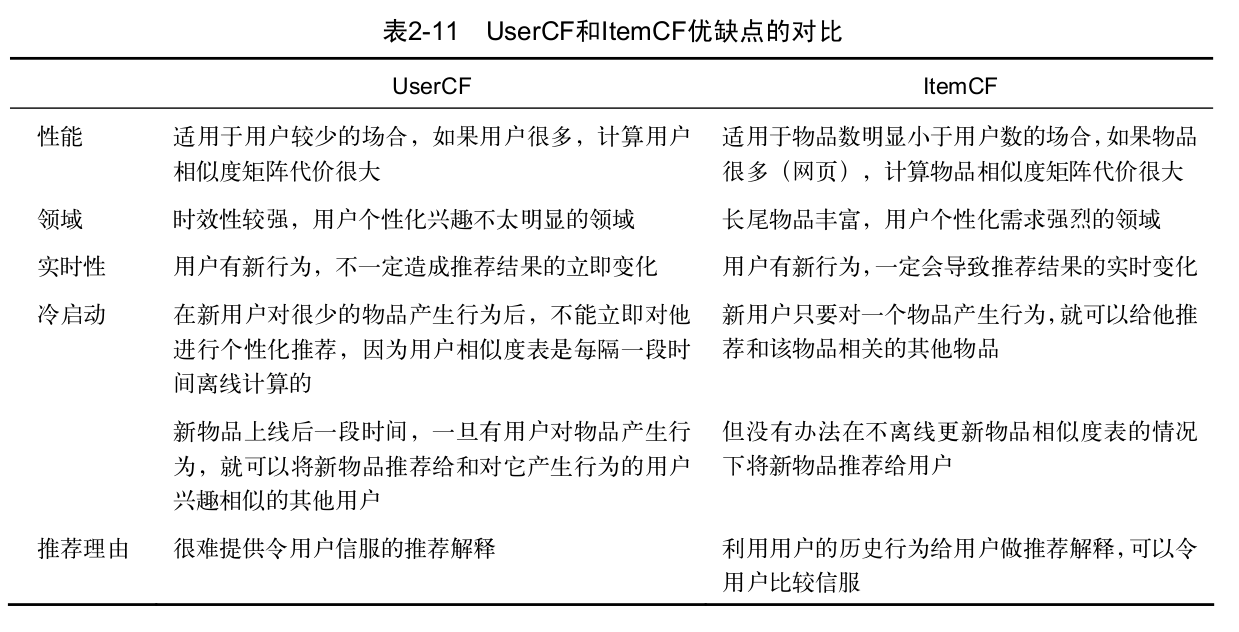
\includegraphics[width = 0.9\textwidth,trim = 0 -0 0 -0,clip]{UserCFandItemCF.png}	  
	\caption{\label{fig: UserCFandItemCF} UserCF 与 ItemCF的对比}
\end{figure} 

协同过滤方法本质还是一种kNN的算法,只不过距离函数采用用户/物品相似度进行度量。


